\documentclass[10pt,a4paper]{article}
\usepackage[utf8]{inputenc}
\usepackage[english]{babel}
\usepackage{amsmath}
\usepackage{amsfonts}
\usepackage{amssymb}
\usepackage{graphicx}
\usepackage{hyperref}

\author{Jakob Zwiener}
\title{Metanome Algorithm Integration}

\begin{document}

\maketitle

\section{Configuration and Execution}
\label{sec_configurationAndExecution}

Metanome supplies a framework to develop data profiling algorithms that integrate into the Metanome tool. Algorthms are packaged in jars that contain a bootstrap class that implements one or several of the specific algorithm interfaces shown in Figure~\ref{fig_algorithmClass}.
\begin{figure}[h]
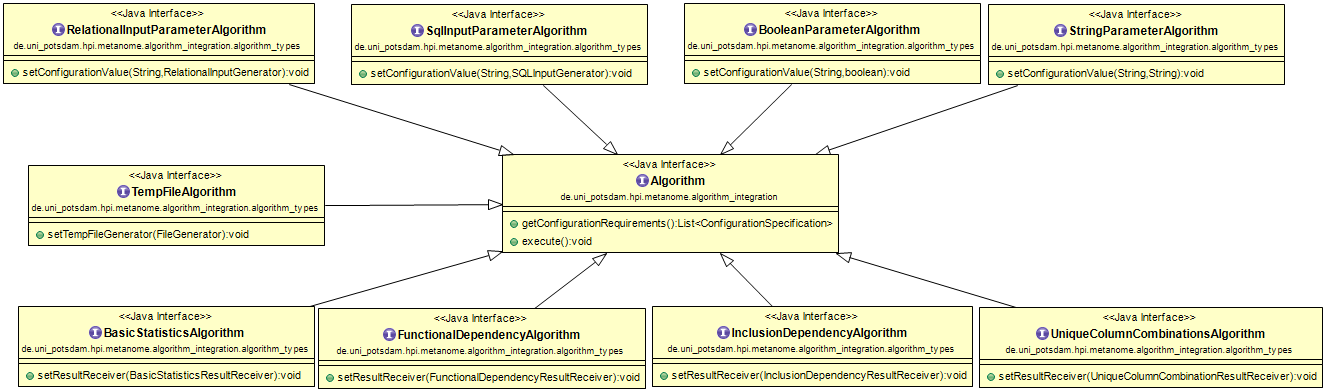
\includegraphics[width=\textwidth]{algorithm_class}
\caption{Algorithm interfaces}
\label{fig_algorithmClass}
\end{figure}
There are interfaces that determine the \texttt{ResultReceiver} of the algorithm and thus the types of results an algorithm can produce. Other interfaces determine the type of parameters that can be set on the algorithm upon configuration. The \texttt{TempFileAlgorithm} interface allows the algorithm to request temporary files from the framework. An algorithm bootstrap class needs to be declared in the manifest of the jar in an \texttt{Algorithm-Bootstrap-Class} tag and needs to implement the following methods:

\begin{itemize}
\item \texttt{List <ConfigurationSpecification> getConfigurationRequirements()}

The algorithm should generate a list of necessary configuration parameters. Configuration parameters that can be requested are shown in Figure~\ref{fig_configurationSpecificationClass}.

\begin{figure}[h]
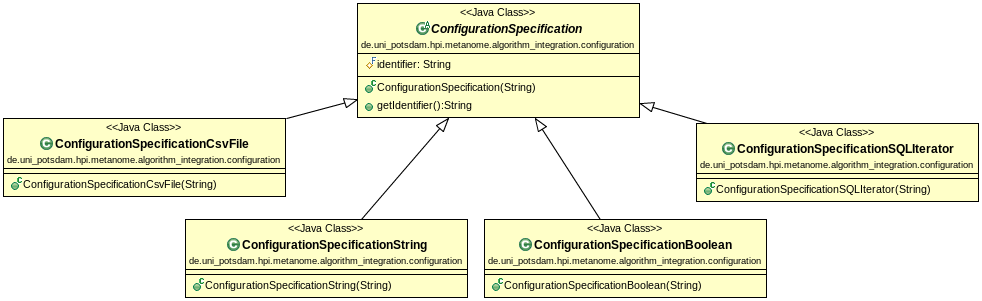
\includegraphics[width=\textwidth]{configurationSpecification_class}
\caption{Configuration specifications}
\label{fig_configurationSpecificationClass}
\end{figure}

\item \texttt{void setConfigurationValue(String, ?)}

The algorithm should receive the results of the requested configuration through the \texttt{setConfigurationValue} methods. Possible configuration values are shown in Figure~\ref{fig_configurationValueClass}. The algorithm needs to declare all interfaces of requested configuration types.

\begin{figure}[h]
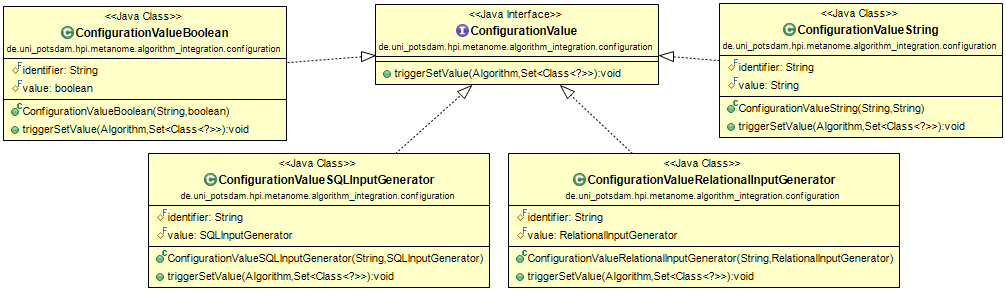
\includegraphics[width=\textwidth]{configurationValue_class}
\caption{Configuration values}
\label{fig_configurationValueClass}
\end{figure}

\item \texttt{void setResultReceiver(ResultReceiver)}

Algorithms generate certain types of results shown in Figure~\ref{fig_resultsClass} and send those to the Metanome tool through a callback.
\begin{figure}[h]
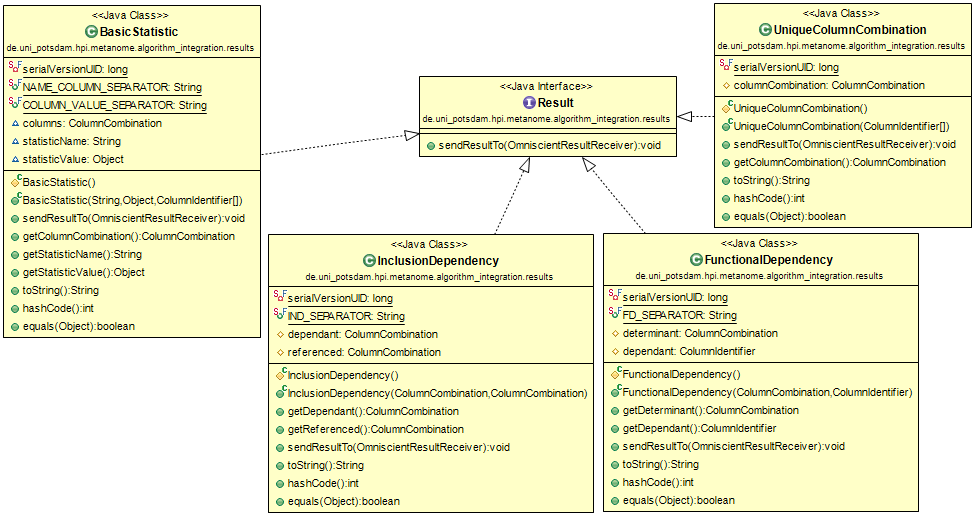
\includegraphics[width=\textwidth]{results_class}
\caption{Results}
\label{fig_resultsClass}
\end{figure}
To enable this one or several \texttt{ResultReceiver} are set on the algorithm, depending on the algorithm type. Existing result receiver are shown in Figure~\ref{fig_resultReceiverClass}.

\begin{figure}[h]
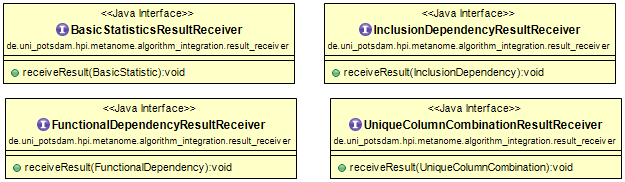
\includegraphics[width=\textwidth]{resultReceiver_class}
\caption{Result receiver}
\label{fig_resultReceiverClass}
\end{figure}

\item \texttt{void execute()}

Algorithm execution can be started by calling the execute method.

\end{itemize}

A typical execution sequence of the configuration and execution of an algorithm in the Metanome tool is shown in Figure~\ref{fig_integrationSequence}.

\begin{figure}[h]
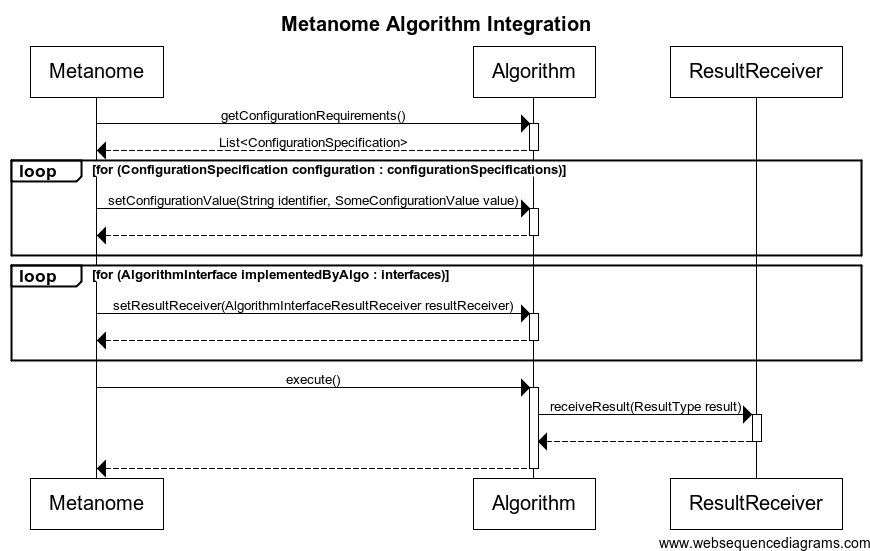
\includegraphics[width=\textwidth]{algorithm_sequence}
\caption{Configuration and execution sequence}
\label{fig_integrationSequence}
\end{figure}

\section{Sample Algorithm}
\label{sec_sampleAlgorithm}

To simplify the development of algorithms for the Metanome tool a maven sample project is provided. Necessary changes to the template are described in the following:

\begin{itemize}
\item Rename the project directory and change the \texttt{groupId}, \texttt{artifactId} and \texttt{name} in the pom.
\item Rename the \texttt{AlgorithmTemplate.java} and \texttt{AlgorithmTemplateTest.java}.
\item Update the algorithm bootstrap class in the \texttt{Algorithm-Bootstrap-Class} tag in the pom.
\item Declare algorithm types in the bootstrap class by implementing one or several of the algorithm interfaces shown in Figure~\ref{fig_algorithmClass}. 
\item Update the package names according to the entries in the pom.
\item Build the algorithm jar with \texttt{mvn package}.
\end{itemize}

\section{Executing Algorithms}
\label{sec_executingAlgortithms}

Algorithms are executed using the Metanome tool. A Metanome installation can be downloaded from the metanome file share\footnote{\url{https://www.hpi.uni-potsdam.de/naumann/sites/metanome/files/}}. The installation contains the Metanome tool and the Jetty web server for execution. Algorithms should be placed in the \texttt{metanome/WEB-INF/classes/algorithms/} directory; input files should be placed in the \texttt{metanome/WEB-INF/classes/inputData/} directory.

\end{document}